\chapter{OpenMP: Synchronisation, Mutual Exclusion}
\label{ch:synchronization}

\section*{Learning Outcomes}
\addcontentsline{toc}{section}{Learning Outcomes}

\begin{enumerate}
    \item Implement thread-specific control flow using conditionals based on thread IDs and understand when manual synchronization is required.
    \item Apply the \texttt{single} directive to execute code once by any available thread, and control implicit barriers using the \texttt{nowait} clause.
    \item Use the \texttt{master} directive to designate thread~0 for specific tasks and understand the absence of implicit barriers.
    \item Insert explicit barriers using \texttt{\#pragma omp barrier} to synchronize thread teams and ensure memory consistency across shared variables.
    \item Implement mutual exclusion using OpenMP locks (\texttt{omp\_lock\_t}) with proper initialization, acquisition, release, and destruction.
    \item Distinguish between race conditions (intentional competition for resources) and data races (unordered conflicting accesses), and use locks to prevent the latter.
    \item Differentiate between mutual exclusion (serialized access) and atomicity (indivisible operations), understanding that neither implies the other.
    \item Apply \texttt{\#pragma omp atomic} for efficient atomic operations on single variables using hardware support.
    \item Design fine-grained locking schemes with proper deadlock avoidance strategies such as consistent lock ordering.
    \item Analyze trade-offs between global locks (simple but limiting concurrency) and fine-grained locks (complex but enabling better parallelism).
\end{enumerate}

\section*{Recap from Previous Lecture}
\addcontentsline{toc}{section}{Recap from Previous Lecture}

\begin{itemize}
    \item Parallelism can be expressed as data parallelism or task parallelism, corresponding broadly to SIMD and MIMD execution styles.
    \item OpenMP provides a shared-memory programming interface for C/C++ and Fortran, based on a fork--join execution model.
    \item Parallel regions and parallel loops can be created using \texttt{\#pragma omp parallel} and \texttt{\#pragma omp parallel for}, with loop iterations distributed across threads.
    \item Execution order in multithreaded programs is nondeterministic, which may lead to unordered outputs and subtle concurrency bugs.
    \item A data race occurs when multiple threads access the same memory location concurrently with at least one write, and such races can be avoided using appropriate data-sharing clauses like \texttt{private} and \texttt{shared}.
\end{itemize}



\section{Thread Control Flow and Synchronization}
\label{sec:thread-control}

This section explores additional OpenMP primitives for \emph{thread-specific control flow}\index{control flow!thread-specific}: situations where some threads execute a piece of code while others do not. 

\begin{ppdefn}
\ppterm{\\Thread-specific control flow}\index{control flow!thread-specific} describes execution in a parallel region where different threads may follow different control paths.
For example, one thread may execute a block (such as initialization) while other threads skip it.
Such divergence is typically driven by the thread ID or other runtime conditions.
It often requires explicit synchronization when threads later depend on results produced by only some threads.
\end{ppdefn}

\subsection{Thread-Specific Control Flow via Conditionals}

Consider a parallel region where every thread needs to know the total number of threads in the team.
The value of \texttt{numt} denotes the number of threads in the \emph{current} OpenMP team.
 For a given parallel region, this value is fixed for the lifetime of that region, so it is wasteful to have every thread redundantly write it. 
\begin{ppprogram}{Reading the value of \texttt{numt}}{prog:tid-read}
\begin{lstlisting}[language=OpenMP]
#include <omp.h>
#include <stdio.h>

int main(void) {
    int numt, tid;

    #pragma omp parallel private(tid)
    {
        tid = omp_get_thread_num();
        numt = omp_get_num_threads();
    }

    return 0;
}
\end{lstlisting}
\end{ppprogram}
One common pattern to remove this redundancy is to use the thread ID to conditionally execute code only on a specific thread.
For example, in Program~\ref{prog:tid-conditional}, only the thread with \texttt{tid==0} (often called the \emph{master thread}) assigns the value of \texttt{numt}.

\begin{ppprogram}{Naive thread-specific control flow using a conditional}{prog:tid-conditional}
\begin{lstlisting}[language=OpenMP]
#include <omp.h>
#include <stdio.h>

int main(void) {
    int numt, tid;

    #pragma omp parallel private(tid)
    {
        tid = omp_get_thread_num();

        if (tid == 0)
            numt = omp_get_num_threads();
    }

    return 0;
}
\end{lstlisting}
\end{ppprogram}

\begin{ppdefn}
\ppterm{\\Control divergence}\index{control divergence} occurs when not all threads execute the same control path.
One thread may perform a setup-like task (e.g., recording the team size), while other threads skip that work.
This code segment shown above~\ref{prog:tid-conditional} is an early glimpse of task-based parallelism: different threads may perform different roles even within the same parallel region.
\end{ppdefn}

\begin{figure}[h]
    \centering
    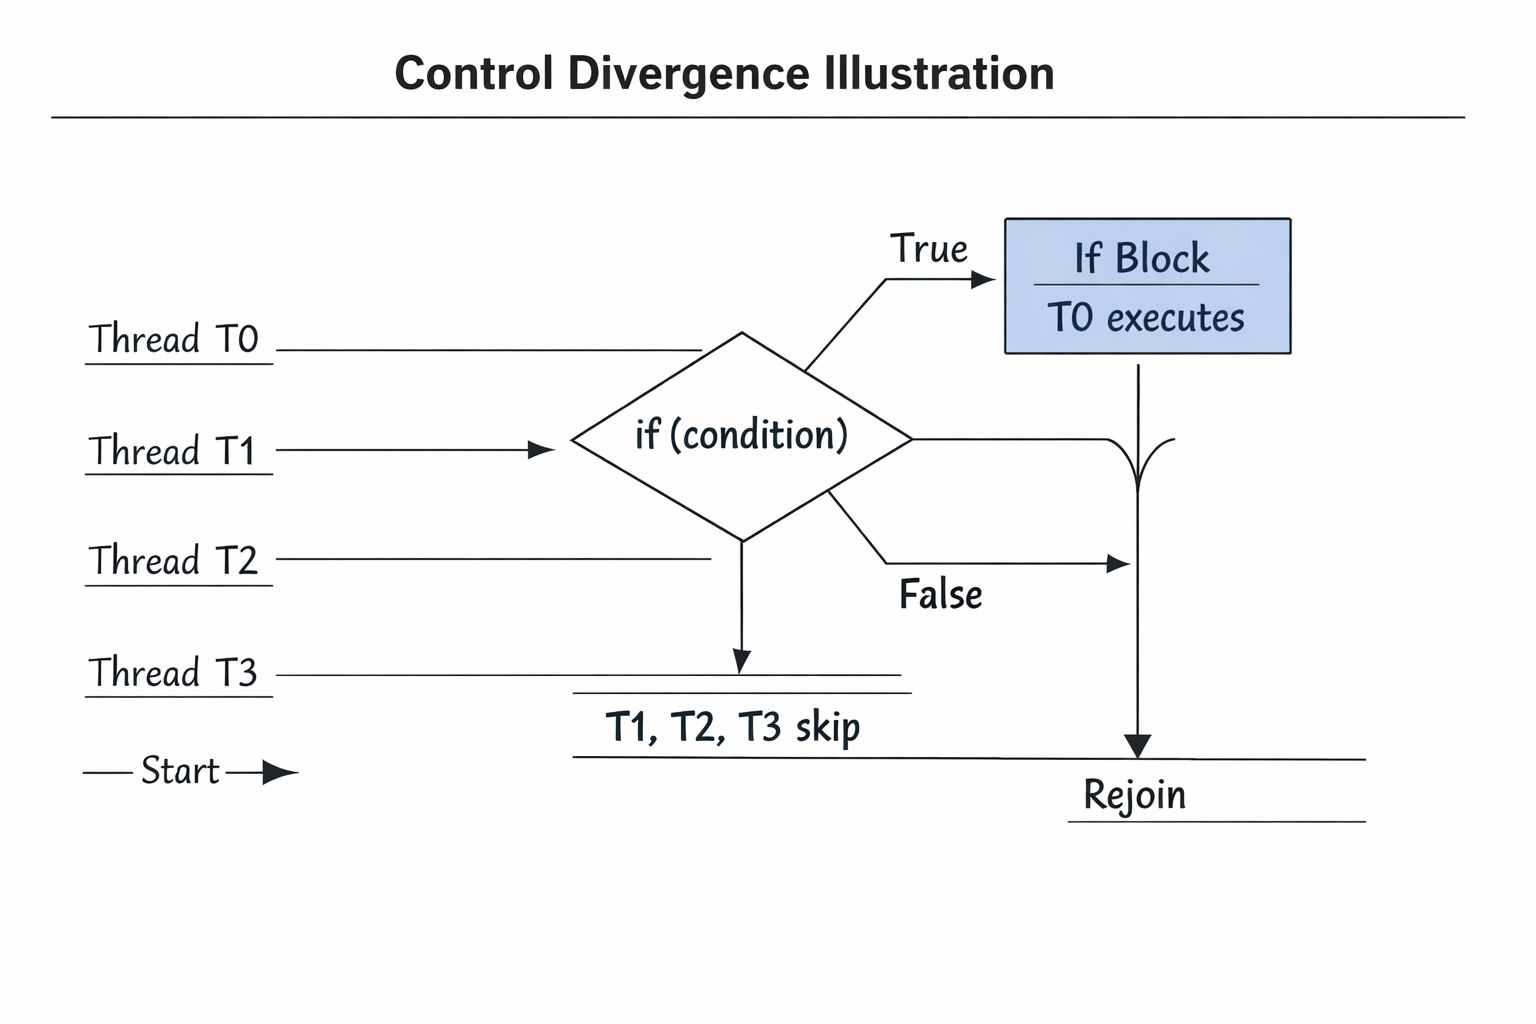
\includegraphics[width=0.75\textwidth]{media/thread_divergence.png}
    \caption{Control divergence: Thread~0 executes the conditional block while other threads skip it.}
    \label{fig:control-divergence}
\end{figure}

\begin{pppitfall}
\\While Program~\ref{prog:tid-conditional} is fine as a \emph{pattern} for ``only one thread should write this shared variable,''
it does \emph{not} by itself guarantee that other threads will see the initialized value at the point they use it.
If we need other threads to read \texttt{numt} immediately afterwards, explicit synchronization is required.
\end{pppitfall}

\subsection{The \texttt{single} Directive}
\label{sec:single-directive}
\index{single directive@\texttt{single} directive}

This raises a natural question: \emph{Given a parallel region, can we ask OpenMP to execute a region using only a single thread and ensuring explicit synchronization?}

Yes. OpenMP provides \texttt{\#pragma omp single}~\cite{openmp-spec}. Exactly one thread in the team (not predetermined; chosen by the runtime) executes the associated block. By default, \texttt{single} also introduces an \emph{implicit barrier}\index{barrier!implicit} at the end of the block, meaning that all other threads wait until the single thread finishes that block.

\begin{figure}[h]
    \centering
    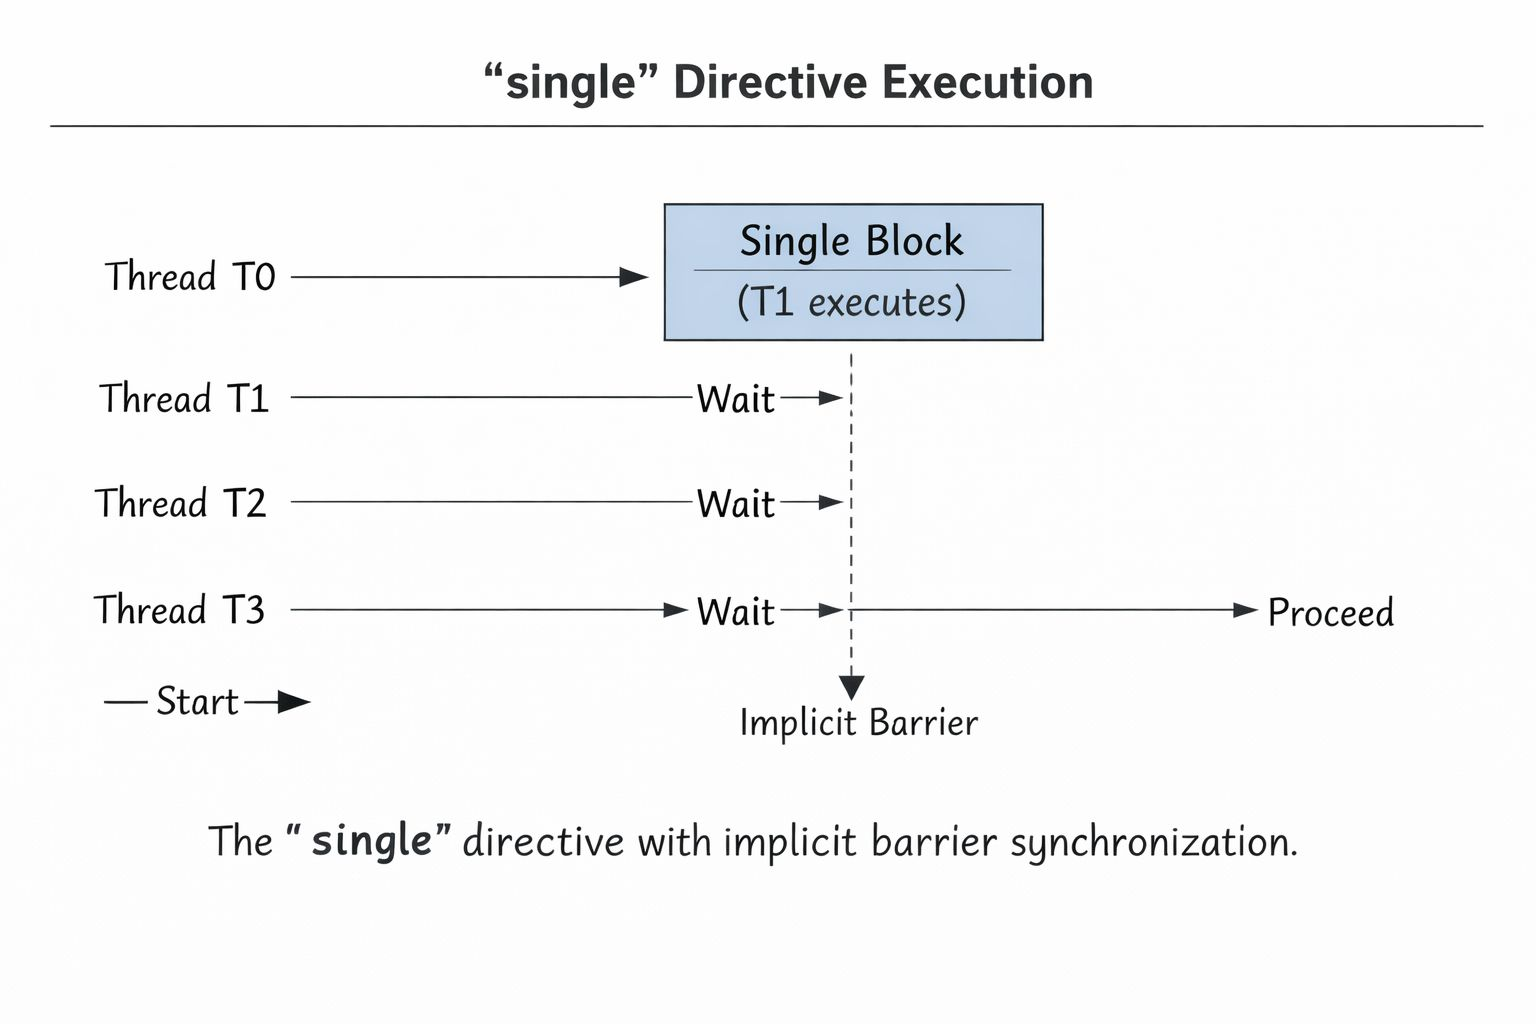
\includegraphics[width=0.75\textwidth]{media/barrier.jpg}
    \caption{Single thread executes the block; other threads wait at the implicit barrier.(Note that the single thread is arbitarily chosen by runtime but the figure shows thread 0 for illustration.)}
    \label{fig:barrier-implicit}
\end{figure}

\begin{ppprogram}{\texttt{omp single} with implicit barrier}{prog:omp-single}
\begin{lstlisting}[language=OpenMP]
#pragma omp single
{
    numt = omp_get_num_threads();
}  /* implicit barrier here */
\end{lstlisting}
\end{ppprogram}

\begin{ppquestion}
\textbf{\\How is \texttt{single} different from a conditional?}

\textbf{Answer:}
\begin{itemize}
    \item \textbf{Work assignment:} \texttt{single} allows any available thread in the team to execute the block; a conditional fixes responsibility to a specific thread ID (often \texttt{tid==0}). If thread~0 is busy, the conditional approach can delay progress unnecessarily.
    \item \textbf{Synchronization:} \texttt{single} has an implicit barrier by default, which makes it a safe ``initialize-once'' mechanism when other threads need the results immediately after the block. A conditional does \emph{not} automatically synchronize.
\end{itemize}
\end{ppquestion}

\subsubsection{The \texttt{nowait} Clause}

Sometimes you want \texttt{single} to perform work by one thread \emph{without forcing all other threads to wait immediately}. For that, OpenMP provides \texttt{nowait}, which removes the implicit barrier at the end of the \texttt{single} block:

\begin{ppprogram}{\texttt{omp single nowait} (no implicit barrier)}{prog:omp-single-nowait}
\begin{lstlisting}[language=OpenMP]
#pragma omp single nowait
{
    numt = omp_get_num_threads();
}
\end{lstlisting}
\end{ppprogram}

\begin{ppnote}
\texttt\\{nowait} is safe only when no other thread requires the results of the \texttt{single} block immediately after it. If they do, you must introduce synchronization later (e.g., an explicit \texttt{barrier} or a different dependency structure).
\end{ppnote}

The \texttt{single} directive must appear \emph{inside} an OpenMP parallel region; outside a parallel region it has no useful semantics (there is no thread team from which to choose a single executor).

\subsection{The \texttt{master} Directive}
\label{sec:master-directive}
\index{master directive@\texttt{master} directive}

There is another way to force \emph{the master thread} (thread~0 of the team) to execute a region: \texttt{\#pragma omp master}.

\begin{ppdefn}
\\In an OpenMP parallel region, each thread has a thread ID in $\{0, 1, \dots, \texttt{numt}-1\}$. The thread with \texttt{tid==0} is referred to as the \ppterm{master thread}\index{master thread} of that team.
\end{ppdefn}


\begin{ppquestion}
\textbf{\\Does \texttt{master} introduce an implicit barrier like \texttt{single}?}

\textbf{Answer:} No. Unlike \texttt{single}, the \texttt{master} directive has \emph{no implicit barrier} at the end.
This is ideal when other threads should continue working without waiting.
\end{ppquestion}

\subsubsection{Comparing Control Flow Mechanisms}

\begin{ppnote}
\textbf{\\When to use each mechanism:}
\begin{itemize}
    \item \textbf{Conditional (\texttt{if (tid==0)}):} Quick-and-dirty thread-specific control flow when you want a fixed thread to do a small action (e.g., update a counter, print a header). You must manage synchronization yourself if others depend on the result.
    \item \textbf{\texttt{single}:} One-time initialization or one-time computation inside a parallel region where \emph{any} thread may do it, and where the implicit barrier is desirable for correctness (or \texttt{nowait} when you do not want to stall the team).
    \item \textbf{\texttt{master}:} Operations that must be executed by the master thread specifically (e.g., interacting with a master-only API, coordinating I/O policies, or maintaining a single ``coordinator'' role). Since there is no implicit barrier, it is ideal when other threads should continue working without waiting.
\end{itemize}
\end{ppnote}

\begin{ppexample}
\ppemph{\\MapReduce analogy.} In distributed systems such as MapReduce, one often describes a \emph{master/coordinator} that schedules work for many \emph{workers}. OpenMP is shared-memory threading (not distributed), but the intuition can still help: using \texttt{master} lets thread~0 act as a coordinator while other threads proceed. The key difference is that in OpenMP the ``master'' is simply \texttt{tid==0} within a thread team, not a separate process.
\end{ppexample}


\begin{ppquestion}
\\When we define the number of threads as 4, does that mean there are 4 worker threads and 1 main thread, or 4 threads including the master thread?

\textbf{Answer:} It is the second option: 4 threads total in the team \emph{including} the master thread (\texttt{tid==0}). Thread IDs will be $0, 1, 2, 3$.
\end{ppquestion}
\subsection{Explicit Synchronization with Barriers}
\label{sec:barriers}
\index{barrier!explicit}

Now suppose we want to add synchronization to the conditional approach so that all threads use \texttt{numt} only after it has been set. This connects directly to the concepts of mutual exclusion and atomicity discussed in Section~\ref{sec:mutual-exclusion}.

\begin{ppdefn}
\\An OpenMP \ppterm{barrier}\index{barrier} is a \emph{team-wide synchronization point}. Every thread in the team must arrive at the barrier before any thread is allowed to proceed past it. In addition, a barrier implies a memory consistency action (a ``flush''\index{flush} of shared variables) so that writes performed before the barrier become visible to reads after the barrier.
\end{ppdefn}


OpenMP provides the directive \texttt{\#pragma omp barrier} for this purpose.

\begin{ppprogram}{Conditional control flow with explicit barrier}{prog:barrier-sync}
\begin{lstlisting}[language=OpenMP]
#include <omp.h>
#include <stdio.h>

int main(void) {
    int numt, tid;

    #pragma omp parallel shared(numt) private(tid)
    {
        tid = omp_get_thread_num();

        if (tid == 0)
            numt = omp_get_num_threads();

        #pragma omp barrier

        // All threads wait here until thread 0 has set numt
        // Now all threads can safely use numt
        printf("hello world %d of %d\n", tid, numt);
    }

    return 0;
}
\end{lstlisting}
\end{ppprogram}

\begin{ppquestion}
\\ Is Program~\ref{prog:barrier-sync} equivalent to \texttt{\#pragma omp master}?

\textbf{Answer:} No. It is best understood as \texttt{master}-like behavior \emph{plus explicit synchronization}. The assignment \texttt{if (tid==0) numt = ...} matches the ``executed by master only'' idea, but the \texttt{barrier} is \emph{not} part of \texttt{master} semantics. In fact, Program~\ref{prog:barrier-sync} is essentially: ``do the assignment on the master thread, then force the whole team to wait until the master is done, then continue.''
\end{ppquestion}

\subsubsection{Barrier Behavior Analysis}

\begin{ppquestion}
\textbf{What changes when we add the barrier?}

\textbf{Answer:} All threads are guaranteed to print using the initialized value of \texttt{numt}.
If the team size is 4, you will see four lines, one per thread, and each line will have \texttt{of 4}.
The \emph{order is not guaranteed} (threads may print in any order), but typical output will look like:
\begin{verbatim}
hello world 0 of 4
hello world 2 of 4
hello world 1 of 4
hello world 3 of 4
\end{verbatim}
\end{ppquestion}

\begin{pppitfall}
\\\textbf{Without the barrier:} If you remove the \texttt{\#pragma omp barrier}, the program contains a race between the master thread writing \texttt{numt} and other threads reading \texttt{numt} for printing. Some threads may print before \texttt{numt} is initialized, so \texttt{numt} may appear as an uninitialized (garbage) value or an unexpected number. This is a classic pitfall: ``only one thread writes'' is not sufficient for correctness unless readers are synchronized with the writer.
\end{pppitfall}

\subsection{Key Takeaways}

This section introduced three mechanisms for thread-specific control flow in OpenMP:
\begin{itemize}
    \item \textbf{Conditionals} (e.g., \texttt{if (tid==0)}) allow specific threads to execute code based on thread ID, but require manual synchronization to ensure data visibility across threads.
    \item \textbf{\texttt{single}} ensures exactly one thread executes a code block, with an implicit barrier by default (removable via \texttt{nowait}), allowing any available thread to perform the work.
    \item \textbf{\texttt{master}} designates thread~0 to execute a code block without any implicit barrier, ideal for coordinator tasks where other threads should continue independently.
    \item \textbf{Explicit barriers} (\texttt{\#pragma omp barrier}) synchronize all threads at a common point, ensuring memory consistency and visibility of shared variable updates across the team.
    \item \textbf{Control divergence} occurs when different threads follow different execution paths, requiring careful synchronization design when threads depend on work performed by only some threads.
\end{itemize}
The next section explores how these synchronization concepts relate to mutual exclusion and atomicity.

\subsection{Exercises}

\begin{ppexercises}
  \ppexercise{If we modify Program~\ref{prog:barrier-sync} to use \texttt{\#pragma omp single} instead of the conditional, compare the behavior with and without \texttt{nowait}.}
  
  \textbf{Answer:} With \texttt{\#pragma omp single}, any thread executes the initialization and an implicit barrier ensures all threads wait. This replaces both the conditional and explicit barrier. With \texttt{nowait}, the behavior becomes similar to the original without a barrier, other threads may print before \texttt{numt} is set, causing undefined behavior.
  
  \ppexercise{Explain why using \texttt{\#pragma omp master} without an explicit barrier can lead to incorrect results when other threads depend on values set by the master.}
  
  \textbf{Answer:} The \texttt{master} directive has no implicit barrier. If other threads proceed immediately to use values set by the master thread, they may read uninitialized or stale data because the master thread may not have completed the assignment yet. An explicit barrier is needed to ensure the master's writes are visible to other threads.
  
\end{ppexercises}

\section{OpenMP Locks}
\label{sec:locks}
\index{locks}

This section studies another important synchronization mechanism in shared-memory parallel programming: \emph{locks}. Locks are used to ensure \textbf{orderly access} to a region of code that must not be executed concurrently by multiple threads. The fundamental property achieved using locks is \textbf{mutual exclusion}, as will be seen in Section~\ref{sec:mutual-exclusion}.

The discussion is motivated by the need to selectively \emph{sequentialize} parts of an otherwise parallel program. While threads are typically free to execute independently and concurrently, certain code regions, called \emph{critical regions}\index{critical region}, must be accessed in a controlled fashion to avoid incorrect behavior.

\begin{ppnote}
\textbf{\\ Relationship to other sections:} This section provides the practical API for mutual exclusion using OpenMP locks. The conceptual treatment appears in Section~\ref{sec:mutual-exclusion}. The \texttt{single} directive introduced in Section~\ref{sec:thread-control} executes a region once; locks enable repeated, serialized execution by all threads.
\end{ppnote}

\subsection{Lock Fundamentals}

\subsubsection{What Is a Lock?}

\begin{ppdefn}
\\ A \ppterm{lock} is an abstraction that protects a specific region of code. Conceptually:
\begin{itemize}
    \item Multiple threads may want to execute the same region of code $C$ (the critical section).
    \item At most one thread is allowed to execute $C$ at any given time.
    \item Other threads must wait until the currently executing thread exits $C$.
\end{itemize}
In simple terms, a lock \emph{locks} a region of code so that only one thread can be inside that region at a time.
\end{ppdefn}

Here, $C$ represents any critical code region that manipulates shared data. For example:
\begin{lstlisting}[language=C11]
// Example critical region C:
omp_set_lock(&mylock);
balance -= amount;      // Read-modify-write on shared variable
omp_unset_lock(&mylock);
\end{lstlisting}

\subsubsection{Locks vs \texttt{single}}
\label{sec:locks-vs-single}

At first glance, locks may appear similar to the OpenMP construct \texttt{\#pragma omp single} (see Section~\ref{sec:single-directive}). However, the semantics are fundamentally different:

\begin{figure}[h]
    \centering
    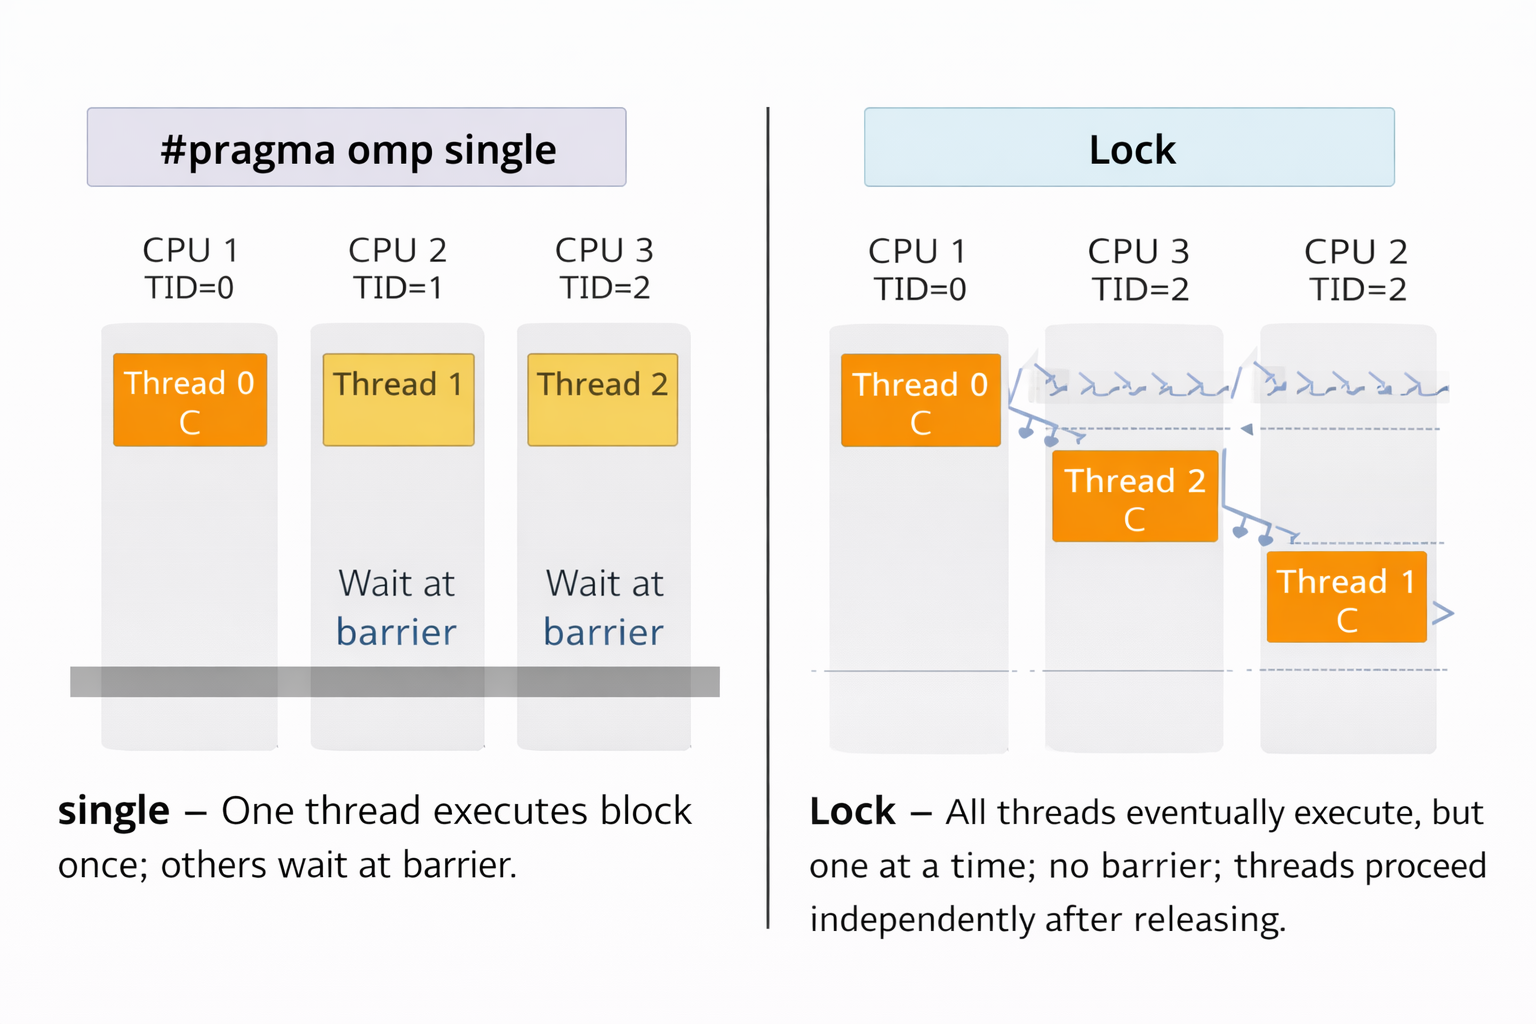
\includegraphics[width=0.8\textwidth]{media/singleVSlock.png}
    \caption{Comparison of \texttt{single} directive (executes once by one thread) versus locks (all threads execute serially, one at a time)}
    \label{fig:locks-vs-single}
\end{figure}

\begin{ppnote}
\\Throughout this section, we use $C$ to denote a generic \emph{critical code region}, a sequence of statements that accesses shared data and must be protected from concurrent execution. For example:
\begin{lstlisting}[language=C11]
// Code region C:
shared_counter++;
shared_sum += local_value;
\end{lstlisting}
\end{ppnote}

\begin{ppkey}
\begin{itemize}
    \item \textbf{\texttt{single}:} The code region $C$ is executed by exactly one thread, and never by the others.
    \item \textbf{Lock:} Every thread \emph{may eventually execute} $C$, but execution is serialized, one thread at a time.
\end{itemize}
Thus, a lock enables \emph{multiple executions in an orderly fashion}, whereas \texttt{single} enforces a \emph{single execution}.
\end{ppkey}

\begin{ppnote}
\\ Importantly, \texttt{single} introduces an implicit barrier at the end (unless \texttt{nowait} is specified), whereas \textbf{locks do not introduce any implicit barrier}. Threads proceed independently after unlocking.
\end{ppnote}

\subsection{Lock Implementation and Behavior}

\subsubsection{Conceptual Model of Locking}

Consider a shared lock variable $V$:
\begin{itemize}
    \item $V$ resides in shared memory.
    \item Initially, $V = 0$ (unlocked).
    \item A thread that sets $V = 1$ acquires the lock.
    \item Releasing the lock resets $V$ to $0$.
\end{itemize}

All threads compete to acquire $V$. The first thread that succeeds enters the critical region $C$. Other threads wait.

\subsubsection{Spin Waiting}

\begin{ppdefn}
\\ In a naive implementation, waiting threads repeatedly check the value of $V$ in a loop. This is called \ppterm{spin waiting} or \ppterm{busy waiting}.
\end{ppdefn}

\begin{ppprogram}{Naive spin lock implementation}{prog:spin-lock}
\begin{lstlisting}[language=C11]
while (V != 0) {
    // spin
}
V = 1;  // acquire lock
\end{lstlisting}
\end{ppprogram}

\begin{pppitfall}
\\ The naive implementation in Program~\ref{prog:spin-lock} has a \emph{race condition}\index{race condition}: multiple threads may simultaneously observe \texttt{V == 0} and both proceed to set \texttt{V = 1}. Real lock implementations use atomic operations (such as compare-and-swap\index{compare-and-swap}, or CAS) to avoid this. This is why the \texttt{omp\_lock\_t} abstraction exists, it handles these low-level details correctly.
\end{pppitfall}

Modern processors and runtimes optimize spin waiting behavior, but the fundamental idea remains: waiting threads repeatedly check the lock state until it becomes available.

\subsubsection{Sequentialization in a Parallel Program}

A natural question arises:

\begin{quote}
\emph{If $n$ threads execute the same region $C$ sequentially using a lock, is this equivalent to executing $n$ copies of $C$ sequentially?}
\end{quote}

\begin{ppkey}
\\ Yes, and that is the point. Locks provide a programming-language-level abstraction that allows the programmer to intentionally serialize execution of a critical region within a parallel program.

Without such an abstraction, threads would execute $C$ concurrently and cause incorrect behavior. Locks give the programmer explicit control over where and how sequentialization occurs.
\end{ppkey}

\subsection{Concurrency Issues and Correctness}

\subsubsection{Fairness, Starvation, and Scheduling}

\begin{pppitfall}
\\ It is possible for a thread to:
\begin{itemize}
    \item Release a lock,
    \item Reach the next iteration,
    \item And re-acquire the lock again before other threads.
\end{itemize}
This can lead to \ppterm{starvation}, where some threads never get a chance to execute a certain code section$C$.
\end{pppitfall}

Whether starvation happens depends on:
\begin{itemize}
    \item The lock implementation,
    \item Scheduling policies,
    \item Hardware and runtime behavior.
\end{itemize}

Designing \emph{fair} synchronization primitives is an active research topic spanning operating systems, architecture, and programming languages.

\subsubsection{Race Conditions vs Data Races}

The lecture emphasizes an important distinction:

\begin{ppdefn}
\begin{description}
    \item[\ppterm{Race condition}:] Multiple threads competing to acquire a resource. This is \emph{intentional} and necessary for locks.
    \item[\ppterm{Data race}:] Concurrent access to shared data where at least one access is a write and accesses are unordered. This is \emph{incorrect}.
\end{description}
\end{ppdefn}

\begin{ppkey}
\\ Locks \textbf{allow race conditions} (competition to acquire the lock) but \textbf{prevent data races} inside the protected region.

Since only one thread executes $C$ at a time, shared variables inside $C$ cannot be concurrently modified.
\end{ppkey}

\subsubsection{How Do Threads Observe Unlocking?}

Threads waiting for a lock repeatedly read the shared lock variable from memory. Conceptually:
\begin{itemize}
    \item The lock variable $V$ is stored at a memory address.
    \item Waiting threads issue repeated read requests for $V$.
    \item When $V$ changes (unlock), threads observe the update and compete to acquire it.
\end{itemize}

The runtime coherence ensures that only one thread succeeds in acquiring the lock, even if multiple threads attempt simultaneously.

\subsection{OpenMP Lock API and Usage}
\label{sec:lock-primitives}

\subsubsection{Lock Primitives}
\index{omp\_lock\_t}\index{omp\_nest\_lock\_t}

OpenMP exposes lock functionality explicitly through library calls~\cite{openmp-spec}. Unlike the directive-based constructs (\texttt{parallel}, \texttt{single}, \texttt{critical}), locks are managed via explicit function calls, giving the programmer fine-grained control.

\subsubsection{Lock Types}

\begin{ppnote}
\\ OpenMP provides two lock types:
\begin{itemize}
    \item \texttt{omp\_lock\_t}: Normal (non-nestable) lock.
    \item \texttt{omp\_nest\_lock\_t}: Nestable lock that allows re-acquisition by the same thread.
\end{itemize}
\end{ppnote}

\subsubsection{Lock API}

\begin{ppprogram}{OpenMP lock API}{prog:lock-api}
\begin{lstlisting}[language=OpenMP]
void omp_init_lock(omp_lock_t *lock);
void omp_set_lock(omp_lock_t *lock);    // acquire
void omp_unset_lock(omp_lock_t *lock);  // release
void omp_destroy_lock(omp_lock_t *lock);

int omp_test_lock(omp_lock_t *lock);    // try-acquire
\end{lstlisting}
\end{ppprogram}

\begin{ppkey}
\\ \texttt{omp\_test\_lock} returns immediately:
\begin{itemize}
    \item Non-zero if the lock was acquired,
    \item Zero otherwise (no blocking).
\end{itemize}
\end{ppkey}

\subsubsection{Using \texttt{omp\_test\_lock}}

\begin{ppprogram}{Using test lock for non-blocking acquisition}{prog:test-lock-usage}
\begin{lstlisting}[language=OpenMP]
int flag = 0;
while (!flag) {
    flag = omp_test_lock(&lock);
    // Optionally do other work while waiting
}
// Lock acquired, proceed with critical section
\end{lstlisting}
\end{ppprogram}

\subsubsection{Complete Lock Example}

\begin{ppexample}
\\ Here is a complete example demonstrating proper lock usage to protect a shared counter:
\end{ppexample}

\begin{ppprogram}{Protecting a shared counter with locks}{prog:lock-counter}
\begin{lstlisting}[language=OpenMP]
#include <omp.h>
#include <stdio.h>

int main() {
    int counter = 0;
    omp_lock_t lock;
    
    omp_init_lock(&lock);
    
    #pragma omp parallel
    {
        for (int i = 0; i < 1000; i++) {
            omp_set_lock(&lock);
            counter++;  // Critical section
            omp_unset_lock(&lock);
        }
    }
    
    omp_destroy_lock(&lock);
    
    printf("Counter = %d\n", counter);
    return 0;
}
\end{lstlisting}
\end{ppprogram}

\begin{ppnote}
\\ Without the lock in Program~\ref{prog:lock-counter}, the increment operation would suffer from lost updates, the final counter value would be unpredictable and less than expected.
\end{ppnote}

\subsection{Key Takeaways}

This section covered the OpenMP lock API for implementing mutual exclusion:
\begin{itemize}
    \item \textbf{Locks vs \texttt{single}:} Locks enable serialized, repeated execution by all threads (each thread eventually executes the critical region), whereas \texttt{single} executes code exactly once by one thread only.
    \item \textbf{OpenMP lock API:} The \texttt{omp\_lock\_t} type with functions \texttt{omp\_init\_lock}, \texttt{omp\_set\_lock}, \texttt{omp\_unset\_lock}, \texttt{omp\_destroy\_lock}, and \texttt{omp\_test\_lock} provide explicit, fine-grained lock management.
    \item \textbf{Race conditions vs data races:} Locks intentionally allow race conditions (threads competing for lock acquisition) but prevent data races inside the protected critical region by ensuring mutual exclusion.
    \item \textbf{No implicit barriers:} Unlike \texttt{single}, locks do not introduce implicit barriers, threads proceed independently after releasing locks, enabling better concurrency.
    \item \textbf{Fairness and starvation:} Lock implementations may be unfair, potentially causing starvation where some threads repeatedly acquire locks while others wait indefinitely; fairness is implementation and scheduler-dependent.
\end{itemize}

\subsection{Exercises}

\begin{ppexercises}
  \ppexercise{Explain why \texttt{omp\_single} cannot replace locks when all threads must eventually execute a critical region.}
  
  \textbf{Answer:} \texttt{omp\_single} executes the enclosed code exactly once, by one thread only. Other threads skip it entirely. In contrast, locks allow every thread to eventually execute the critical region, but in a serialized manner (one at a time). If all threads need to perform the same operation on shared data (e.g., each adding their contribution), \texttt{single} would only capture one thread's contribution, losing the others.
  
  \ppexercise{Consider a small OpenMP program where threads increment a shared counter:
  \begin{itemize}
      \item First without locks (observe incorrect result),
      \item Then using \texttt{omp\_lock\_t}.
  \end{itemize}
  Compile with \texttt{gcc -fopenmp} and run multiple times. Explain the difference in results.}
  
  \textbf{Answer:} Without locks, concurrent increments cause lost updates due to race conditions. If 4 threads each increment 1000 times, the expected result is 4000, but you'll observe values like 1203 or 2891, different on each run. With \texttt{omp\_lock\_t} protecting the increment, mutual exclusion ensures the final counter is consistently 4000. The lock serializes access, preventing overlapping read-modify-write cycles.
  
  \ppexercise{Consider a lock that is unfair. Explain how starvation may arise with a looped critical region. Explain a timeline showing a possible execution where thread~0 acquires the lock 10 times before thread~1 acquires it once.}
  
  \textbf{Answer:} In an unfair lock, thread~0 can release the lock, loop back, and immediately reacquire it before thread~1 (waiting at the lock) gets scheduled. The timeline shows thread~0 repeatedly: acquire→execute→release→loop→acquire, while thread~1 remains spinning. This starvation occurs when the scheduler or lock implementation favors the releasing thread, violating fairness guarantees.
  
  \ppexercise{Classify the following as race condition, data race, both, or neither, and justify your answer:
  \begin{itemize}
      \item Two threads calling \texttt{omp\_set\_lock} on the same lock
      \item Two threads incrementing the same variable without synchronization
      \item Two threads reading the same constant
      \item One thread writing while another reads without synchronization
  \end{itemize}}
  
  \textbf{Answer:} (1) Race condition only, threads compete for the lock, but this is intentional and correctly handled by the lock implementation. (2) Both, threads race to acquire/update the variable (race condition) and have concurrent conflicting accesses (data race). (3) Neither, concurrent reads of immutable data are safe. (4) Data race only, conflicting accesses (write and read) without ordering, though one could argue the write/read also constitute a race condition.
  
  \ppexercise{Compare and contrast using \texttt{\#pragma omp critical} with explicit locks via \texttt{omp\_lock\_t}. When would you prefer one over the other? Consider both correctness and performance.}
  
  \textbf{Answer:} \texttt{critical} is simpler, the runtime manages the lock implicitly, and unnamed \texttt{critical} sections share one global lock. \texttt{omp\_lock\_t} provides fine-grained control: multiple independent locks, conditional acquisition (\texttt{test\_lock}), and explicit lock passing. Prefer \texttt{critical} for simplicity when one global critical section suffices. Prefer explicit locks for: multiple independent critical regions, non-blocking acquisition patterns, or when lock handles need to be managed dynamically. Performance is similar for single locks, but explicit locks enable better concurrency with multiple locks.
\end{ppexercises}

\section{Mutual Exclusion and Atomicity}
\label{sec:mutual-exclusion}
\index{mutual exclusion}\index{atomicity}

This section explores the critical distinction between mutual exclusion and atomicity, two fundamental concepts in parallel programming that are often conflated but represent distinct guarantees. Understanding this distinction is essential for writing correct concurrent code, building on the synchronization primitives introduced in Section~\ref{sec:thread-control}.

\subsection{What is Mutual Exclusion?}

\begin{ppdefn}
\ppterm{\\Mutual exclusion}\index{mutual exclusion!definition} ensures that only one thread at a time executes a designated \ppterm{critical section}\index{critical section}. Programmers typically use a \ppterm{lock}\index{lock}/\ppterm{unlock} protocol to serialize access among threads that compete to run the same code region. See Section~\ref{sec:locks} for detailed coverage of OpenMP lock primitives.
\end{ppdefn}

Suppose there are $n$ threads competing to execute code region~$C$. Using a lock, the programmer sequentializes access so that a single thread executes the critical section while the others wait.

\begin{figure}[H]
    \centering
    % Prefer an external graphic if available; otherwise fall back to the boxed diagram.
    \IfFileExists{media/mutual_exclusion.png}{%
        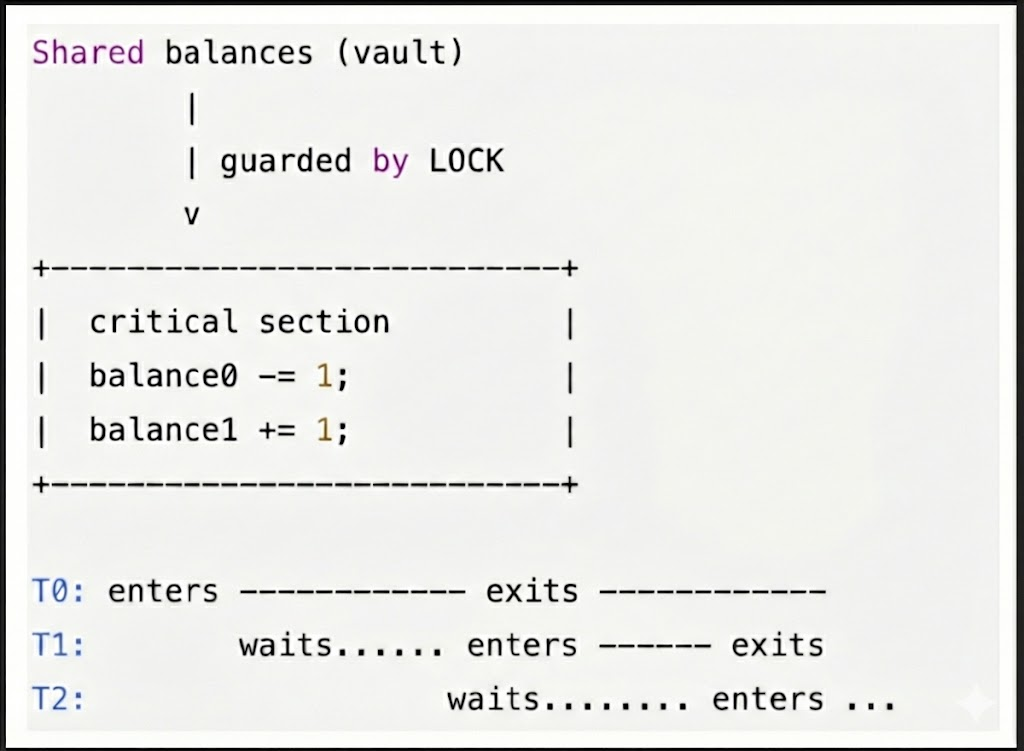
\includegraphics[width=0.7\textwidth]{media/mutual_exclusion.png}
        \\ A critical code region is guarded by a lock. Thread $T_0$ acquires lock \texttt{v} and enters the region; threads $T_1$ and $T_2$ wait. Waiting threads spin (poll) on \texttt{v}. When $T_0$ exits, it releases \texttt{v}; then $T_1$ acquires it and enters, while the remaining threads continue to wait. In this way, execution of the critical section is serialized.
    }{%
        \fbox{\parbox{0.7\textwidth}{\centering 
        \textbf{Mutual Exclusion Diagram}\\[0.5em]
        }}
    }
    \caption{Mutual exclusion using locks}
    \label{fig:mutual_exclusion}
\end{figure}

\subsection{Mutual Exclusion vs Atomicity}

\begin{pppitfall}
\textbf{\\ Do not conflate \ppterm{mutual exclusion} with \ppterm{atomicity}.}
\begin{itemize}
    \item \textbf{Mutual exclusion:} Only one thread executes the critical section at a time; the running thread can still be preempted by the operating system.
    \item \textbf{Atomicity:} A tagged sequence of instructions appears as a single, indivisible step to all observers, it cannot be interrupted or interleaved.
\end{itemize}
Neither property implies the other.
\end{pppitfall}

\begin{ppkey}
\\ Atomicity presents an indivisible view of a sequence of actions; mutual exclusion merely serializes entry into a region. They are related but distinct guarantees.
\end{ppkey}

\subsection{Atomicity Without Mutual Exclusion}

\begin{ppexample}
\ppemph{\\
Atomicity without mutual exclusion.} In the following code block we see that the increment operation itself is atomic, but threads are not excluded from running concurrently, many threads can perform the atomic increment at the same time without lost updates.
\end{ppexample}

\begin{ppprogram}{OpenMP atomic increment (no mutual exclusion)}{prog:atomic-no-me}
\begin{lstlisting}[language=OpenMP]
#include <omp.h>
#include <stdio.h>

int main() {
    long long hits = 0;

    #pragma omp parallel
    {
        // Many threads execute concurrently (no mutual exclusion),
        // but each increment is atomic (no lost updates).
        #pragma omp atomic
        hits++;
    }

    printf("hits = %lld\n", hits);
    return 0;
}
\end{lstlisting}
\end{ppprogram}

In this example, multiple threads can reach the \texttt{\#pragma omp atomic}\index{atomic directive@\texttt{atomic} directive} directive simultaneously. Each individual increment is atomic (no partial updates or lost writes), but the threads are not mutually excluded from executing concurrently.

\begin{ppnote}
\textbf{\\ Hardware support:} The \texttt{atomic} directive typically compiles to hardware atomic instructions (e.g., \texttt{lock xadd} on x86). This is more efficient than acquiring a lock for simple operations like increment, decrement, or compare-and-swap.
\end{ppnote}

\subsection{Mutual Exclusion Without Atomicity}

\begin{ppexample}
\ppemph{\\ Mutual exclusion without atomicity.} In the following code block each individual balance update is protected by a per-account lock (mutual exclusion holds per account), but the transfer as a whole is not atomic because the debit and credit occur in two separate locked regions. Other threads can observe intermediate state.
\end{ppexample}

\begin{ppprogram}{Per-account locks: transfer not atomic as a whole}{prog:me-no-atomic}
\begin{lstlisting}[language=OpenMP]
#include <omp.h>

// Conceptual example
extern omp_lock_t acct_lock[];
extern long long balance[];

// Transfer money from -> to (WRONG if atomic transfer is required)
void transfer(int from, int to, long long amount) {
    omp_set_lock(&acct_lock[from]);
    balance[from] -= amount;   // debit
    omp_unset_lock(&acct_lock[from]);

    // Another thread can observe the debit before the credit happens.

    omp_set_lock(&acct_lock[to]);
    balance[to] += amount;     // credit
    omp_unset_lock(&acct_lock[to]);
}
\end{lstlisting}
\end{ppprogram}

\begin{pppitfall}
\\ In Program~\ref{prog:me-no-atomic}, the invariant ``total money is conserved'' can appear violated to an observer who reads both accounts between the debit and credit. The individual operations have mutual exclusion, but the composite transfer lacks atomicity.
\end{pppitfall}

\subsection{Achieving Both: A Bank Transfer Example}
\label{sec:bank-transfer}
\index{bank transfer example}

To make a transfer truly atomic (as well as mutually exclusive), we must hold locks on \emph{both} accounts for the duration of the entire operation. This example demonstrates the practical application of locks covered in Section~\ref{sec:locks}.

\begin{ppnote}
\textbf{\\ Memory allocation note:} The code uses \texttt{calloc()}\index{calloc()} rather than \texttt{malloc()}. Both return a contiguous block of memory; the key difference is that \texttt{calloc} zero-initializes. Whether \texttt{calloc} is slower depends on the allocator/OS (zeroing may be optimized); do not assume performance characteristics without measurement.
\end{ppnote}

\begin{ppprogram}{Correct atomic transfer using a global lock}{prog:atomic-transfer}
\begin{lstlisting}[language=OpenMP]
#include <stdio.h>
#include <stdlib.h>
#include <omp.h>

int main() {
    const int N_ACCTS = 8;
    const int N_TXNS = 2000000;

    long long *balance = (long long *)calloc(N_ACCTS, sizeof(long long));
    if (!balance) return 1;

    // Initialize all accounts
    for (int i = 0; i < N_ACCTS; i++) {
        balance[i] = 1000;
    }

    omp_lock_t ledger_lock;
    omp_init_lock(&ledger_lock);

    double t0 = omp_get_wtime();

    #pragma omp parallel
    {
        unsigned int seed = (unsigned int)omp_get_thread_num();

        #pragma omp for schedule(static)
        for (int k = 0; k < N_TXNS; k++) {
            int from = (int)(rand_r(&seed) % N_ACCTS);
            int to = (int)(rand_r(&seed) % N_ACCTS);
            if (from == to) continue;

            long long amount = (long long)(rand_r(&seed) % 5);

            // Critical section via an explicit lock
            omp_set_lock(&ledger_lock);

            balance[from] -= amount;
            balance[to] += amount;

            omp_unset_lock(&ledger_lock);
        }
    }

    double t1 = omp_get_wtime();

    omp_destroy_lock(&ledger_lock);

    // Check conservation invariant
    long long total = 0;
    for (int i = 0; i < N_ACCTS; i++)
        total += balance[i];

    printf("Initial total = %lld\n", N_ACCTS * 1000LL);
    printf("Final total   = %lld\n", total);
    printf("Elapsed time  = %f seconds\n", t1 - t0);

    free(balance);
    return 0;
}
\end{lstlisting}
\end{ppprogram}

\begin{ppnote}
\textbf{\\ Key observations from this example:}
\begin{itemize}
    \item The example models concurrent access to shared state: multiple threads perform ``transfers'' between bank accounts.
    \item Without synchronization, updates to shared balances can interleave unpredictably, producing non-deterministic results.
    \item Each transfer conceptually performs a read--modify--write on two shared memory locations: \texttt{balance[from]} and \texttt{balance[to]}.
    \item A data race occurs when two threads access the same location concurrently and at least one access is a write, with no ordering enforced.
\end{itemize}
\end{ppnote}

\begin{ppkey}
\textbf{\\ Correctness specification (invariants and post-condition):}
\begin{itemize}
    \item Desired invariant: the sum of all balances should remain constant (``conservation of money'').
    \item Each valid transfer subtracts \texttt{amount} from one account and adds the same \texttt{amount} to another.
    \item If every transfer is applied atomically as a pair, then total money is preserved.
\end{itemize}
\end{ppkey}


\subsection{Key Takeaways}

This section distinguished two fundamental but often conflated concepts:
\begin{itemize}
    \item \textbf{Mutual exclusion vs atomicity are distinct:} Mutual exclusion serializes access (one thread at a time) but doesn't guarantee atomicity; atomicity makes operations appear indivisible but doesn't require mutual exclusion. Neither property implies the other.
    \item \textbf{Atomicity without mutual exclusion:} \texttt{\#pragma omp atomic} provides atomic operations (like increment) where multiple threads can execute concurrently without lost updates, using hardware atomic instructions rather than locks.
    \item \textbf{Mutual exclusion without atomicity:} Per-resource locks provide mutual exclusion on individual resources, but composite operations spanning multiple resources (like bank transfers) are not atomic unless all involved resources are locked together.
    \item \textbf{Achieving both:} To make multi-variable operations both mutually exclusive and atomic, hold locks on all involved resources for the entire operation duration, as demonstrated in the bank transfer example with a global lock.
    \item \textbf{Performance trade-offs:} Global locks ensure correctness but limit concurrency; fine-grained locking with proper deadlock prevention (e.g., lock ordering) enables better parallelism for operations on disjoint resource sets.
\end{itemize}
Section~\ref{sec:locks} provides the detailed API for implementing these patterns.

\subsection{Exercises}

\begin{ppexercises}
  \ppexercise{Explain why \texttt{\#pragma omp atomic} cannot replace locks when you need to atomically update multiple variables.}
  
  \textbf{Answer:} \texttt{atomic} operates on a single memory location and single operation (e.g., increment, update). It cannot make a compound operation (like \texttt{balance[from] -= amount; balance[to] += amount;}) atomic. Between the two atomic operations, another thread could observe intermediate state where money has been debited but not yet credited, violating invariants. Locks protect the entire critical section as one atomic unit.
  
  \ppexercise{If we modify Program~\ref{prog:atomic-transfer} to use per-account locks instead of a global lock, what additional care is needed to avoid deadlock? (Hint: consider lock ordering.)}
  
  \textbf{Answer:} With per-account locks, thread~A transferring from account~1 to account~2 might hold lock~1 and wait for lock~2, while thread~B transferring from account~2 to account~1 holds lock~2 and waits for lock~1, classic deadlock. Solution: enforce a global lock ordering, such as always acquiring the lock for the lower-numbered account first. If \texttt{from < to}, acquire locks in order \texttt{[from, to]}; otherwise \texttt{[to, from]}. This breaks the circular wait condition.
  
  \ppexercise{Consider a scenario where threads only read account balances without modifying them. Is mutual exclusion still necessary? What about atomicity? Justify your answer.}
  
  \textbf{Answer:} If threads only read and no thread writes, mutual exclusion is not necessary, concurrent reads are safe. However, atomicity concerns remain if balance values are multi-word (e.g., 64-bit on 32-bit systems). A reader might observe a partially updated value if a writer (in another part of the program) is simultaneously updating. If the data is truly read-only (immutable), neither mutual exclusion nor special atomicity handling is needed.
  
  \ppexercise{Classify the following operations as requiring mutual exclusion, atomicity, both, or neither:
  \begin{itemize}
      \item Incrementing a shared counter
      \item Reading a 64-bit value on a 32-bit architecture
      \item Swapping two elements in an array
      \item Appending to a log file
  \end{itemize}}
  
  \textbf{Answer:} (1) Both, atomicity ensures the read-modify-write is indivisible; mutual exclusion ensures only one thread modifies at a time (though \texttt{atomic} alone can suffice). (2) Atomicity only, need to ensure the read is not torn across two 32-bit reads; no write occurring so mutual exclusion not needed. (3) Both, swapping requires reading and writing two locations atomically to prevent other threads from observing inconsistent state. (4) Both, file append involves multiple operations (seek to end, write) that must be atomic and mutually exclusive to prevent interleaved writes.
\end{ppexercises}

\section*{References}
\addcontentsline{toc}{section}{References}
See the OpenMP Specification~\cite{openmp-spec} for authoritative documentation on all directives, lock primitives, atomic operations, and other synchronization constructs discussed in this chapter. For comprehensive coverage of parallel programming concepts and OpenMP, refer to Pacheco~\cite{pacheco2011} and Kumar~\cite{kumar-parallel}.

\section*{Contributions}
\addcontentsline{toc}{section}{Contributions}

This chapter was developed through collaborative efforts of multiple contributors.

\subsection*{Amber Agarwal (2023CS50625)}
Thread Control Flow and Synchronization (Section~\ref{sec:thread-control}: subsections on conditionals, \texttt{single} directive, \texttt{master} directive, and barriers)

\subsection*{Aryan Datir (2023CS10216)}
OpenMP Locks (Section~\ref{sec:locks}: subsections on lock fundamentals, implementation, concurrency issues, and API usage)

\subsection*{Anoop Singh (2023CS10459)}
Mutual Exclusion and Atomicity (Section~\ref{sec:mutual-exclusion}: subsections on mutual exclusion definition, comparison with atomicity, and bank transfer example)

\subsection*{Arinjay Singhal (2023CS10041)}
Key Takeaways and Exercises subsections in Section~\ref{sec:thread-control}, Section~\ref{sec:locks}, and Section~\ref{sec:mutual-exclusion}; Code implementations throughout the chapter

\subsection*{Akhilesh Agrawal (2023CS51192)}
Learning outcomes and Recap 
